\section[Studentische Mitbestimmung]{Studentische Mitbestimmung~I\\Die verfasste Studierendenschaft und die \\studentische Selbstverwaltung}
\label{studmit}

\begin{center}
    	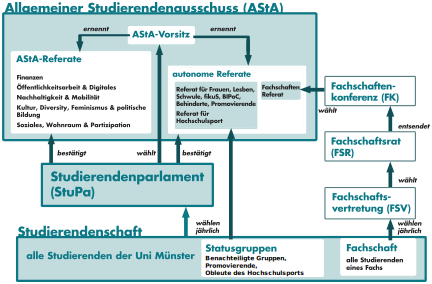
\includegraphics[width=.55\textwidth]{res/verfasste_studierendenschaft_neu.pdf}
	
	\begin{minipage}{0.25\textwidth}
		\footnotesize
		\begin{center}
			\large\textbf{Service des AStA}
		\end{center}
		
		\medskip
				
		Der AStA bietet aktuell folgende Services an:
				
		\smallskip

		\textbf{Verleih} von Lastenfahrrädern, Bullis, Laptops, Musikanlagen
		
		\textbf{Kooperationen} Leihothek Münster, Fahrradwerkstatt, Grüne Kiste
		
		\textbf{Beglaubigte Kopien} von Dokumenten
		
		\textbf{BAföG- und Sozialberatung}
		
		\textbf{Semesterticket und Kultursemesterticket}
		
		\textbf{Beitragserstattungen und Sozialdarlehen}
		
		\textbf{Rechtsberatung kostenlos u. professionell}
		
		\textbf{Babysitting- und Wohnbörse}
		
		\textbf{Sprachkurse}
		
	        \textbf{Kostenlose Fahrradpumpen}
            	
		\textbf{AStA-Druckerei} Arbeiten, Poster etc.
		
		\medskip
		Weitere Informationen auf: \url{https://www.asta.ms}
	\end{minipage}
\end{center}

\begin{multicols*}{2}
Studierende haben grundsätzlich die Möglichkeit an zwei Gebieten der Universität demokratisch teilzuhaben: in der studentischen und akademischen Selbstverwaltung.
Die verfasste Studierendenschaft ist eine gesetzlich vorgeschriebene Organisation der Studierenden und bildet somit die studentische Selbstverwaltung. Jede Person, die an der Uni studiert, ist automatisch Teil dieser Studierendenschaft. Sie hat eine große Anzahl an Aufgaben, die im Hochschulgesetz festgeschrieben sind, sowie finanzielle Mittel von mehr als zehn Millionen Euro jährlich. 
Einmal im Jahr finden die studentischen Wahlen statt, wo z.B. das Studierendenparlament und die Fachschaftsvertretungen neu gewählt werden. 

\paragraph{StuPa}
Studierendenparlament, wird einmal jährlich via Listen gewählt, die teilweise Verbindungen zu Parteien haben. Wählt den AStA mittels Koalitionsbildung. Tagt öffentlich im 1-2 Wochentakt. 


\paragraph{AStA}
Allgemeine Studierenden-Ausschuss, quasi die Regierung der Studierendenschaft. Vertritt sie nach außen, verwaltet die finanziellen Mittel und ist in unterschiedliche themenbezogene Referate (wie Ministerien) gegliedert. Finanziert Semesterticket, Serviceangebote des AStA (siehe Kasten), sowie Serviceangebote der Fachschaften. Autonome Referate werden von der jeweiligen Statusgruppe gewählt und arbeiten daran, das Studium und die Lebensbedingungen für diese Gruppe besser zu gestalten.


\paragraph{FS}
Fachschaft, alle für einen Studiengang eingeschriebenen Studierenden. Ihre Gremien sind Teil der Studierendenschaft. "Fachschaft" wird umgangssprachlich auch verwendet für den FSR und Fachschaftsraum.

Gremien der Fachschaften sind: Die Fachschaftsvertretungen~(FSV), werden jährlich zusammen mit dem StuPa von allen Mitgliedern einer FS gewählt. Die FSVen wählen und kontrollieren den jeweiligen Fachschaftsrat~(FSR), der diverse Angebote auf Fachbereichsebene umsetzt, siehe \cref{fsphys:sec}.

\emph{Die Fachschaft Physik trifft sich aktuell jeden Mittwoch um 18~Uhr im Fachschaftsraum oder online.
Die Sitzungen sind grundsätzlich öffentlich und neue Gesichter sind immer gerne gesehen!}


%\subsection{Das Fachschaftenreferat}
%Das AStA-Fachschaftenreferat ist ein Autonomes Referat des AStA. Es leitet die wöchentliche Fachschaftenkonferenz (FK), in der sich Vertreter der Fachschaftsräte austauschen, und gibt Hilfestellungen für Fachschaften.


\fibelsig{Jan K., Friedrich, Justus, Benedikt B.}
\end{multicols*}


\clearpage


\section*{Studentische Mitbestimmung~II\\Die universitären Strukturen und die \\akademische Selbstverwaltung}
\begin{multicols*}{2}
\begin{quote}
	\textit{Wäre es da nicht doch einfacher, die Regierung löste das Volk auf und wählte ein anderes?}

	\hfill--- Bertold Brecht
\end{quote}
Die Universität selbst ist ebenfalls demokratisch aufgebaut. Dabei werden die Gremien durch die Statusgruppen der Universität, die Studierenden, die Mitarbeiter und die Professoren nach festen Verhältnissen gebildet; die Entsendung geschieht jeweils durch Wahl innerhalb der Statusgruppe.
Die Professoren haben in der Regel absolute Mehrheit. Seit einigen Jahren werden die wichtigsten Entscheidungen im Hochschulrat getroffen, welcher viele externe Mitglieder beinhaltet.


\includegraphics[width=\columnwidth]{res/uni_strukturen.png}


\paragraph{FBR}
Der Fachbereichsrat ist an einem Fachbereich, also auch in der Physik, das wichtigste Gremium.
Hier wird über die wichtigen Entscheidungen im Fachbereich abgestimmt sowie Berufungskommissionen eingerichtet und der Studienbeirat eingesetzt, um die Prüfungsordnungen und deren stetige Verbesserung zu diskutieren.
Die studentischen FBR-Mitglieder (3 reguläre Mitglieder und 3 Stellvertreter) werden im Sommersemester von den Studierenden am Fachbereich gewählt. Diese Wahlen finden zeitgleich mit den Wahlen der verfassten Studierendenschaft statt. 
Sie stehen euch gerne mit Rat zur Verfügung; ihr könnt sie, wie auch die studentischen Mitglieder des Studienbeirats, über die Fachschaft erreichen, um auf Verbesserungen oder Missstände im Studium hinzuweisen.


\paragraph{SHK-Vertretung}
Die SHK-Vertretung wird mit dem FBR zusammen von der Studierendenschaft gewählt und vertritt die Studentischen Hilfskräfte an der Uni. Sie kann gewerkschaftliche Aufgaben übernehmen und Auskunft universitärer Stellen einfordern.


\paragraph{SBR}
Der Studienbeirat wird vom Fachbereichsrat besetzt und hat genauso viele studentische wie nicht-studentische Mitglieder. Im SBR werden Prüfungsordnungsänderungen abgestimmt, bevor sie im FBR thematisiert werden. Außerdem verfügt der SBR über an die Lehrverbesserung gebundene Gelder, die Qualitätsverbesserungsmittel des Fachbereiches.


\paragraph{Senat}
Der Senat ist das wichtigste Gremium der akademischen Selbstverwaltung; hier werden Entscheidungen über Berufungen von Professoren, die Prüfungsordnungen der Fachbereiche und vieles weitere, was die gesamte Uni betrifft, getroffen.
So wird hier auch der Haushaltsplan der Universität von der eingesetzten Finanzkommission erstellt.
Die Senatswahl wird ebenfalls meistens gemeinsam mit den anderen Wahlen abgehalten.


\paragraph{Rektorat}
Das Rektorat ist die Leitung der Uni, welche auch die Verwaltung und das Studierendensekretariat betreut.
Aktueller Rektor ist Herr Prof.\ Johannes Wessels (aus dem Institut für Kernphysik).
Das Rektorat wird unter Aufsicht des Senats vom Hochschulrat gewählt und führt die Vorgaben des Senats und Hochschulrates aus.


\paragraph{HSR}
Der Hochschulrat gibt die Ziele und Richtungen der Universität vor. Er ist zum Großteil aus hochschulexternen Mitgliedern besetzt. Selbst der Senat unterliegt seiner Entscheidungsfindung.


\fibelsig{Friedrich, Justus, Jan K., Benedikt B.}
\end{multicols*}
